\section{Hiện thực ứng dụng}
\subsection{Thủ tục INSERT/UPDATE/DELETE dữ liệu vào 1 bảng dữ liệu}
\textbf{Bảng dữ liệu được chọn:} bảng NhanVien 
\subsubsection{Thủ tục INSERT}

\textbf{Mô tả thủ tục:} Thủ tục có nhiệm vụ thực hiện lệnh thêm vào bảng NhanVien thông tin của nhân viên. Thủ tục hoạt động qua hai quá trình: 
\begin{itemize}
    \item [--] Đầu tiên là kiểm tra định dạng của các tham số được truyền vào, nếu sai định dạng thì sẽ thông báo lỗi và ngừng việc thực hiện thủ tục.
    \item [--] Cuối cùng, sau khi đảm bảo về định dạng, thủ tục sẽ thêm vào bảng NhanVien một thực thể NhanVien mới, với các giá trị là các tham số được cung cấp.
\end{itemize} 

\textbf{Input:} 
\begin{itemize}
    \item [--] Tham số p\_MaNV, có kiểu \texttt{CHAR(6)} 
    \item [--] Tham số p\_Ho, có kiểu \texttt{NVARCHAR(10)} 
    \item [--] Tham số p\_TenLot, có kiểu \texttt{NVARCHAR(10)} 
    \item [--] Tham số p\_Ten, có kiểu \texttt{NVARCHAR(10)} 
    \item [--] Tham số p\_GioiTinh, có kiểu \texttt{ENUM('Nam', 'Nữ', 'Khác')} 
    \item [--] Tham số p\_Email, có kiểu \texttt{VARCHAR(100)} 
    \item [--] Tham số p\_LuongTheoGio, có kiểu \texttt{DECIMAL(10, 2)} 
    \item [--] Tham số p\_MaPhongBan, có kiểu \texttt{CHAR(6)} 
\end{itemize}

\textbf{Output:} Không có.
\textbf{Câu lệnh tạo thủ tục}:
\begin{minted}{mysql}
CREATE PROCEDURE ThemNhanVien(
    IN p_MaNV CHAR(6),
    IN p_Ho NVARCHAR(10),
    IN p_TenLot NVARCHAR(10),
    IN p_Ten NVARCHAR(10),
    IN p_GioiTinh ENUM('Nam', 'Nữ', 'Khác'),
    IN p_Email VARCHAR(100),
    IN p_LuongTheoGio DECIMAL(10, 2),
    IN p_MaPhongBan CHAR(6)
)
\end{minted}
\begin{minted}[firstnumber=11]{mysql}
BEGIN
    -- Kiểm tra dữ liệu hợp lệ
    IF p_MaNV NOT REGEXP '^NV[0-9]{4}$' THEN
        SIGNAL SQLSTATE '45000' SET MESSAGE_TEXT = 'Mã nhân viên phải có định dạng NVxxxx, với 4 chữ số đằng sau';
    END IF;
    IF p_Ho REGEXP '[^a-zA-ZÀ-ỹ ]' THEN
        SIGNAL SQLSTATE '45000' SET MESSAGE_TEXT = 'Họ không được chứa số hoặc ký tự đặc biệt.';
    END IF;
    IF p_TenLot IS NOT NULL AND p_TenLot REGEXP '[^a-zA-ZÀ-ỹ ]' THEN
        SIGNAL SQLSTATE '45000' SET MESSAGE_TEXT = 'Tên lót không được chứa số hoặc ký tự đặc biệt.';
    END IF;
    IF p_Ten REGEXP '[^a-zA-ZÀ-ỹ ]' THEN
        SIGNAL SQLSTATE '45000' SET MESSAGE_TEXT = 'Tên không được chứa số hoặc ký tự đặc biệt.';
    END IF;
    IF p_Email NOT REGEXP '^[a-zA-Z0-9._%+-]+@[a-zA-Z0-9.-]+\.[a-zA-Z]{2,}$' THEN
        SIGNAL SQLSTATE '45000' SET MESSAGE_TEXT = 'Email không đúng định dạng.';
    END IF;
    -- Kiểm tra sự tồn tại của MaPhongBan trong bảng PhongBan
    IF NOT EXISTS (SELECT 1 FROM PhongBan WHERE MaPhongBan = p_MaPhongBan) THEN
        SIGNAL SQLSTATE '45000' SET MESSAGE_TEXT = 'Mã phòng ban không tồn tại.';
    END IF;
    IF p_LuongTheoGio <= 0 THEN
        SIGNAL SQLSTATE '45000' SET MESSAGE_TEXT = 'Lương theo giờ phải lớn hơn 0.';
    END IF;

    -- Thêm nhân viên
    INSERT INTO NhanVien (MaNV, Ho, TenLot, Ten, GioiTinh, Email, LuongTheoGio, MaPhongBan)
    VALUES (p_MaNV, p_Ho, p_TenLot, p_Ten, p_GioiTinh, p_Email, p_LuongTheoGio, p_MaPhongBan);
END //
\end{minted}

\newpage
Một vài câu lệnh thực thi trường hợp báo lỗi
\begin{figure}[H]
    \centering
    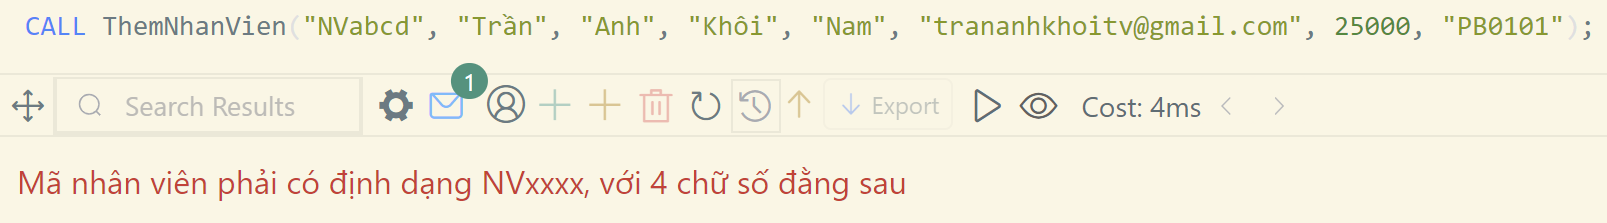
\includegraphics[width=\linewidth]{content/images/ThemNhanVien_LoiMaNV.png}
    \caption{Sử dụng thủ tục ThemNhanVien nhưng sai định dạng MaNV}
    \label{fig:ThemNhanVien_LoiMaNV}
\end{figure}
\begin{figure}[H]
    \centering
    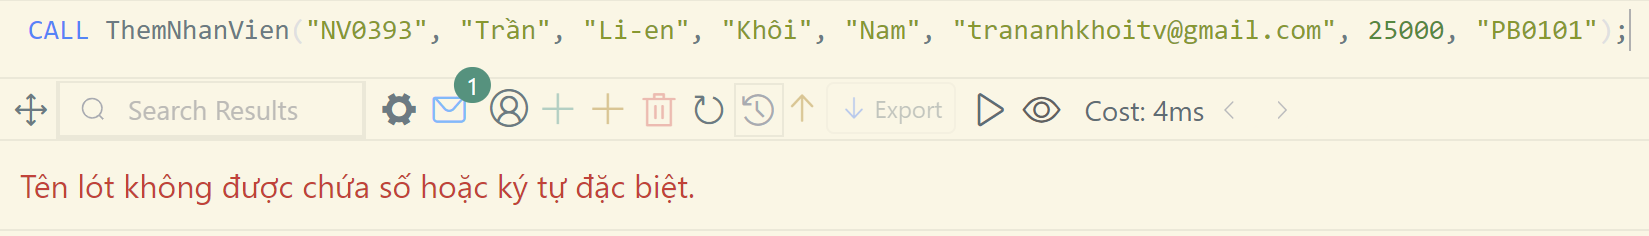
\includegraphics[width=\linewidth]{content/images/ThemNhanVien_LoiTenLot.png}
    \caption{Sử dụng thủ tục ThemNhanVien nhưng sai định dạng TenLoi}
    \label{fig:ThemNhanVien_LoiTenLot}
\end{figure}
\begin{figure}[H]
    \centering
    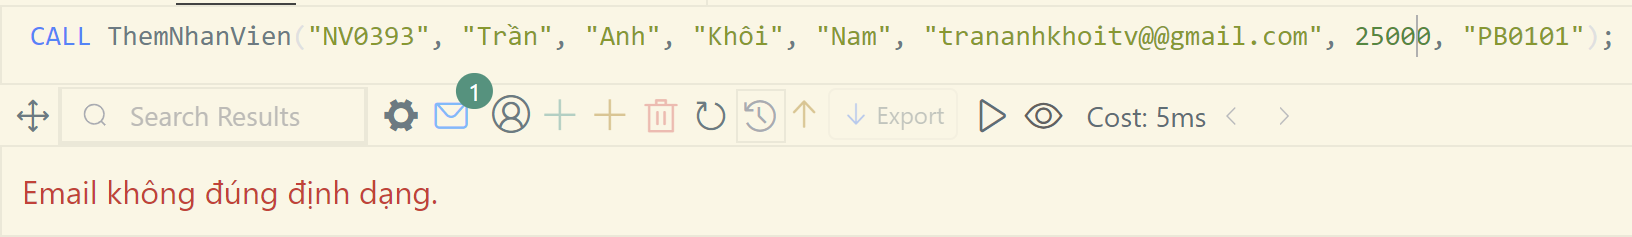
\includegraphics[width=\linewidth]{content/images/ThemNhanVien_LoiEmail.png}
    \caption{Sử dụng thủ tục ThemNhanVien nhưng sai định dạng Email}
    \label{fig:ThemNhanVien_LoiEmail}
\end{figure}
\begin{figure}[H]
    \centering
    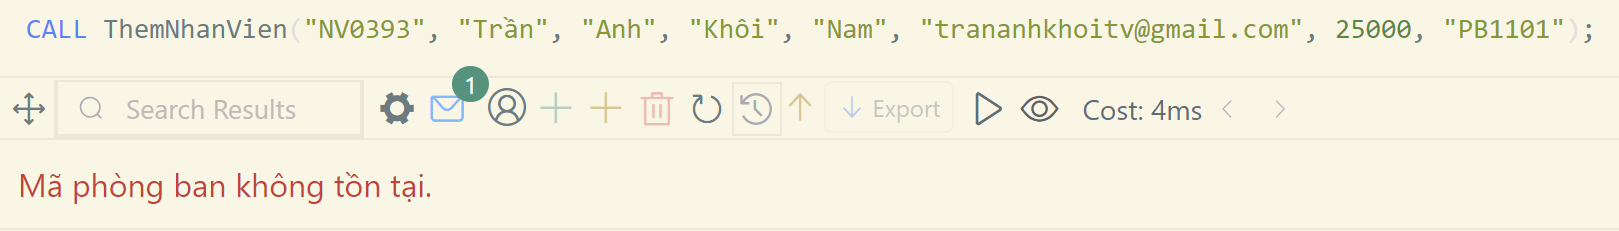
\includegraphics[width=\linewidth]{content/images/ThemNhanVien_LoiPhongBan.png}
    \caption{Sử dụng thủ tục ThemNhanVien nhưng mã phòng ban cung cấp không tồn tại}
    \label{fig:ThemNhanVien_LoiPhongBan}
\end{figure}

Câu lệnh thực thi thủ tục trường hợp đúng:
\begin{figure}[H]
    \centering
    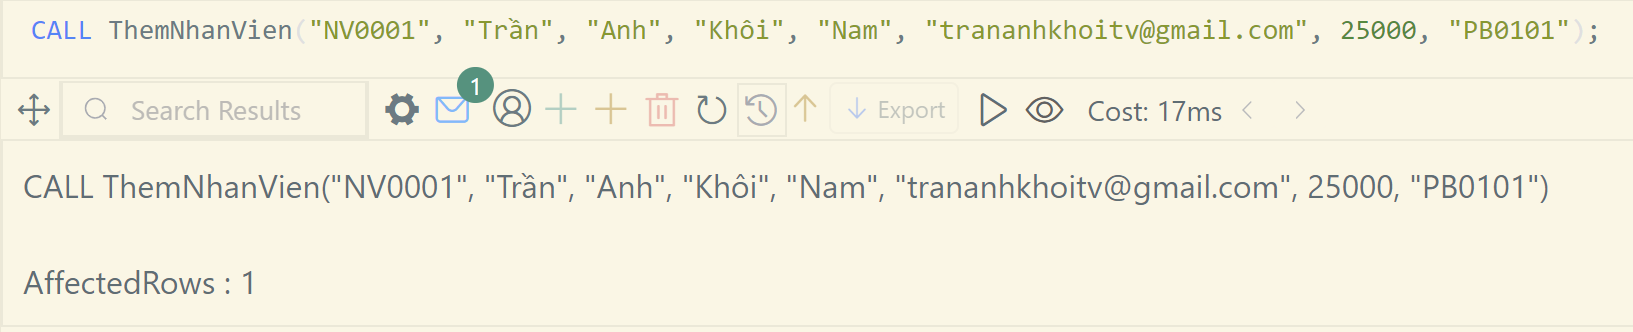
\includegraphics[width=\linewidth]{content/images/ThemNhanVien_ThanhCong.png}
    \caption{Sử dụng thủ tục ThemNhanVien với các tham số đúng định dạng}
    \label{fig:ThemNhanVien_ThanhCong}
\end{figure}

\newpage
\subsubsection{Thủ tục UPDATE}
\textbf{Mô tả thủ tục:} Thủ tục có nhiệm vụ thực hiện lệnh cập nhật một thực thể trong bảng NhanVien. Thủ tục hoạt động qua hai quá trình: 
\begin{itemize}
    \item [--] Đầu tiên là kiểm tra định dạng của các tham số được truyền vào, nếu sai định dạng thì sẽ thông báo lỗi và ngừng việc thực hiện thủ tục.
    \item [--] Cuối cùng, sau khi đảm bảo về định dạng, thủ tục sẽ thêm vào bảng NhanVien một thực thể NhanVien mới, với các giá trị là các tham số được cung cấp.
\end{itemize} 

\textbf{Input:} 
\begin{itemize}
    \item [--] Tham số p\_MaNV, có kiểu \texttt{CHAR(6)}
    \item [--] Tham số p\_Ho, có kiểu \texttt{NVARCHAR(10)}
    \item [--] Tham số p\_TenLot, có kiểu \texttt{NVARCHAR(10)}
    \item [--] Tham số p\_Ten, có kiểu \texttt{NVARCHAR(10)}
    \item [--] Tham số p\_GioiTinh, có kiểu \texttt{ENUM('Nam', 'Nữ', 'Khác')}
    \item [--] Tham số p\_Email, có kiểu \texttt{VARCHAR(100)}
    \item [--] Tham số p\_HeSoPhatDiTre, có kiểu \texttt{DECIMAL(5, 2)}
    \item [--] Tham số p\_HeSoPhatVangKhongPhep, có kiểu \texttt{DECIMAL(5, 2)}
    \item [--] Tham số p\_SoNgayNghi, có kiểu \texttt{INT}
    \item [--] Tham số p\_LuongTheoGio, có kiểu \texttt{DECIMAL(10, 2)}
    \item [--] Tham số p\_MaPhongBan, có kiểu \texttt{CHAR(6)}
\end{itemize}

\textbf{Output:} Không có.

\textbf{Câu lệnh tạo thủ tục}:
\begin{minted}{mysql}
CREATE PROCEDURE SuaNhanVien(
    IN p_MaNV CHAR(6),
    IN p_Ho NVARCHAR(10),
    IN p_TenLot NVARCHAR(10),
    IN p_Ten NVARCHAR(10),
    IN p_GioiTinh ENUM('Nam', 'Nữ', 'Khác'),
    IN p_Email VARCHAR(100),
    IN p_HeSoPhatDiTre DECIMAL(5, 2),
    IN p_HeSoPhatVangKhongPhep DECIMAL(5, 2),
    IN p_SoNgayNghi INT,
    IN p_LuongTheoGio DECIMAL(10, 2),
    IN p_MaPhongBan CHAR(6)
)
\end{minted}
\begin{minted}[firstnumber=14]{mysql}
    BEGIN
    -- Kiểm tra dữ liệu hợp lệ
    IF p_MaNV NOT REGEXP '^NV[0-9]{4}$' THEN
        SIGNAL SQLSTATE '45000' SET MESSAGE_TEXT = 'Mã nhân viên phải có định dạng NVxxxx, với 4 chữ số đằng sau';
    END IF;
    -- Kiểm tra sự tồn tại của nhân viên trong bảng NhanVien
    IF NOT EXISTS (SELECT 1 FROM NhanVien WHERE MaNV = p_MaNV) THEN
        SIGNAL SQLSTATE '45000' SET MESSAGE_TEXT = 'Nhân viên với mã này không tồn tại.';
    END IF;
    IF p_Ho REGEXP '[^a-zA-ZÀ-ỹ ]' THEN
        SIGNAL SQLSTATE '45000' SET MESSAGE_TEXT = 'Họ không được chứa số hoặc ký tự đặc biệt.';
    END IF;
    IF p_TenLot IS NOT NULL AND p_TenLot REGEXP '[^a-zA-ZÀ-ỹ ]' THEN
        SIGNAL SQLSTATE '45000' SET MESSAGE_TEXT = 'Tên lót không được chứa số hoặc ký tự đặc biệt.';
    END IF;

    IF p_Ten REGEXP '[^a-zA-ZÀ-ỹ ]' THEN
        SIGNAL SQLSTATE '45000' SET MESSAGE_TEXT = 'Tên không được chứa số hoặc ký tự đặc biệt.';
    END IF;
    IF p_Email NOT REGEXP '^[a-zA-Z0-9._%+-]+@[a-zA-Z0-9.-]+\.[a-zA-Z]{2,}$' THEN
        SIGNAL SQLSTATE '45000' SET MESSAGE_TEXT = 'Email không đúng định dạng.';
    END IF;
    -- Kiểm tra sự tồn tại của MaPhongBan trong bảng PhongBan
    IF NOT EXISTS (SELECT 1 FROM PhongBan WHERE MaPhongBan = p_MaPhongBan) THEN
        SIGNAL SQLSTATE '45000' SET MESSAGE_TEXT = 'Mã phòng ban không tồn tại.';
    END IF;
    IF p_LuongTheoGio <= 0 THEN
        SIGNAL SQLSTATE '45000' SET MESSAGE_TEXT = 'Lương theo giờ phải lớn hơn 0.';
    END IF;
    IF p_HeSoPhatDiTre < 0 THEN
    SIGNAL SQLSTATE '45000' SET MESSAGE_TEXT = 'Hệ số phạt đi trễ phải lớn hơn hoặc bằng 0.';
    END IF;
\end{minted}
\begin{minted}[firstnumber=46]{mysql}
    IF p_HeSoPhatVangKhongPhep < 0 THEN
    SIGNAL SQLSTATE '45000' SET MESSAGE_TEXT = 'Hệ số phạt vắng không phép phải lớn hơn hoặc bằng 0.';
    END IF;
    IF p_SoNgayNghi < 0 THEN
    SIGNAL SQLSTATE '45000' SET MESSAGE_TEXT = 'Số ngày nghỉ phải lớn hơn hoặc bằng 0.';
    END IF;
    -- Sửa thông tin nhân viên
    UPDATE NhanVien
    SET Ho = p_Ho,
        TenLot = p_TenLot,
        Ten = p_Ten,
        GioiTinh = p_GioiTinh,
        Email = p_Email,
        HeSoPhatDiTre = p_HeSoPhatDiTre,
        HeSoPhatVangKhongPhep = p_HeSoPhatVangKhongPhep,
        SoNgayNghi = p_SoNgayNghi,
        LuongTheoGio = p_LuongTheoGio,
        MaPhongBan = p_MaPhongBan
    WHERE MaNV = p_MaNV;
END //
\end{minted}

\newpage
Một vài câu lệnh thực thi trường hợp báo lỗi
\begin{figure}[H]
    \centering
    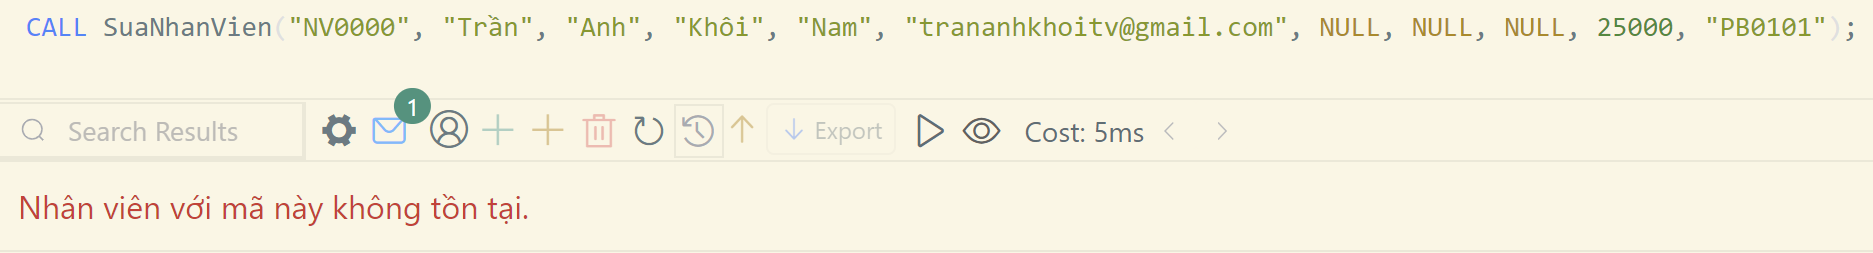
\includegraphics[width=\linewidth]{content/images/SuaNhanVien_MaNVKhongTonTai.png}
    \caption{Sử dụng thủ tục SuaNhanVien trong trường hợp MaNV không tồn tại}
    \label{fig:SuaNhanVien_MaNVKhongTonTai}
\end{figure}
\begin{figure}[H]
    \centering
    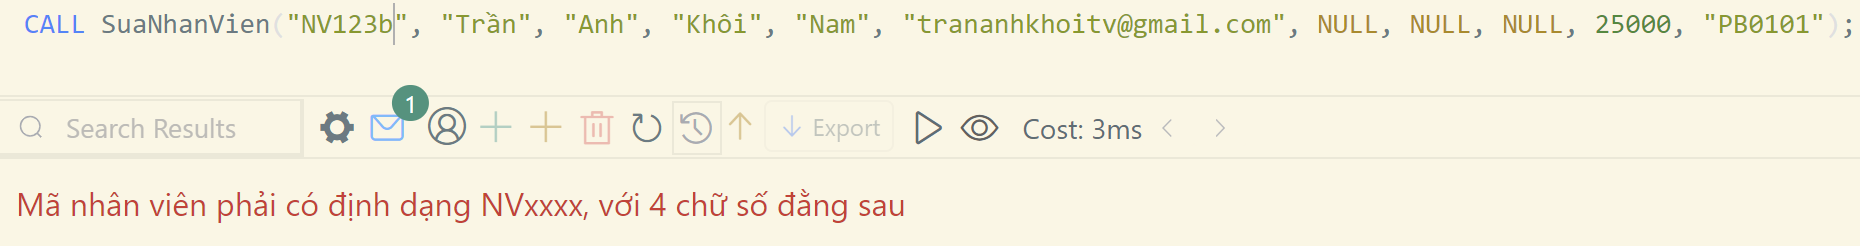
\includegraphics[width=\linewidth]{content/images/SuaNhanVien_MaNVFail.png}
    \caption{Sử dụng thủ tục SuaNhanVien trong trường hợp MaNV sai định dạng}
    \label{fig:SuaNhanVien_MaNVFail}
\end{figure}
\begin{figure}[H]
    \centering
    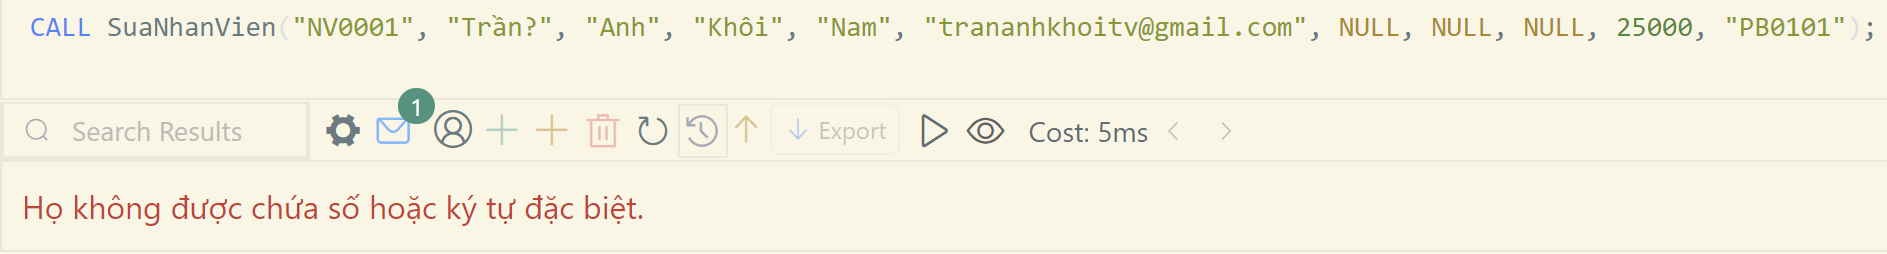
\includegraphics[width=\linewidth]{content/images/SuaNhanVien_HoSaiDinhDang.png}
    \caption{Sử dụng thủ tục SuaNhanVien trong trường hợp Họ sai định dạng}
    \label{fig:SuaNhanVien_HoSaiDinhDang}
\end{figure}
\begin{figure}[H]
    \centering
    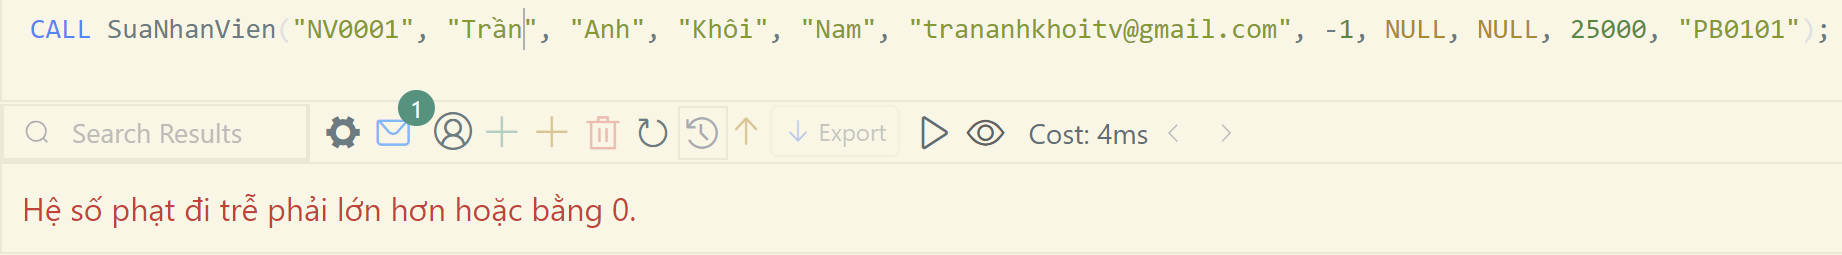
\includegraphics[width=\linewidth]{content/images/SuaNhanVien_HeSoTreFail.png}
    \caption{Sử dụng thủ tục SuaNhanVien trong trường hợp HeSoPhatDiTre bé hơn 0}
    \label{fig:SuaNhanVien_HeSoTreFail}
\end{figure}

\newpage
Câu lệnh thực thi thủ tục trường hợp đúng:
\begin{figure}[H]
    \centering
    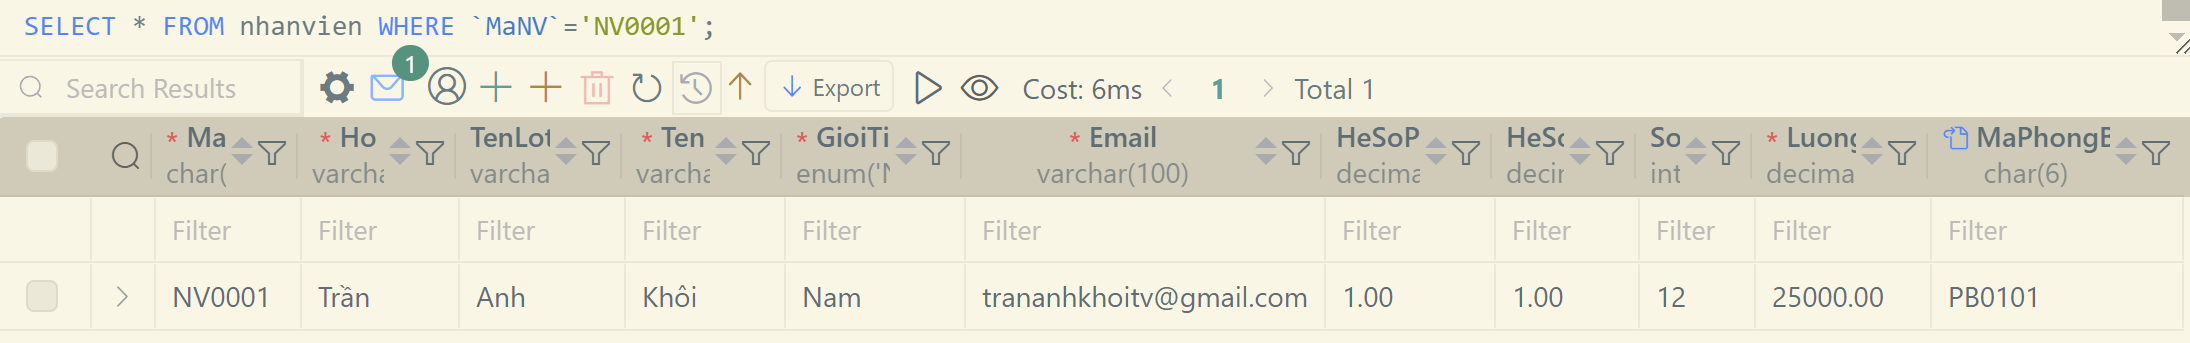
\includegraphics[width=\linewidth]{content/images/SuaNhanVien_Before.png}
    \caption{Trước khi sử dụng thủ tục SuaNhanVien}
    \label{fig:SuaNhanVien_Before}
\end{figure}
\begin{figure}[H]
    \centering
    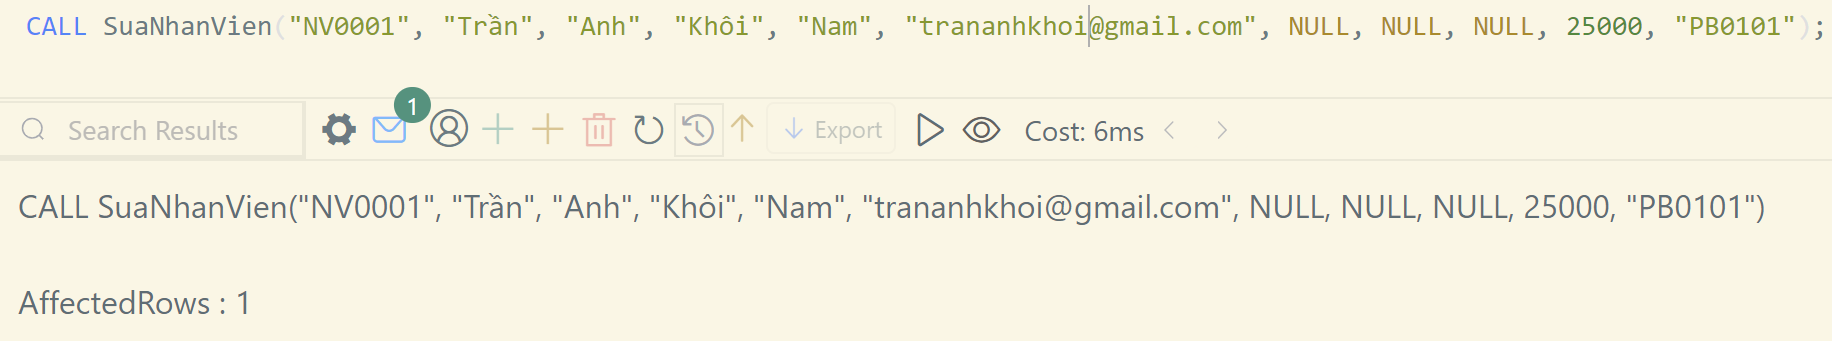
\includegraphics[width=\linewidth]{content/images/SuaNhanVien_ThanhCong.png}
    \caption{Sử dụng thủ tục SuaNhanVien thành công}
    \label{fig:SuaNhanVien_ThanhCong}
\end{figure}
\begin{figure}[H]
    \centering
    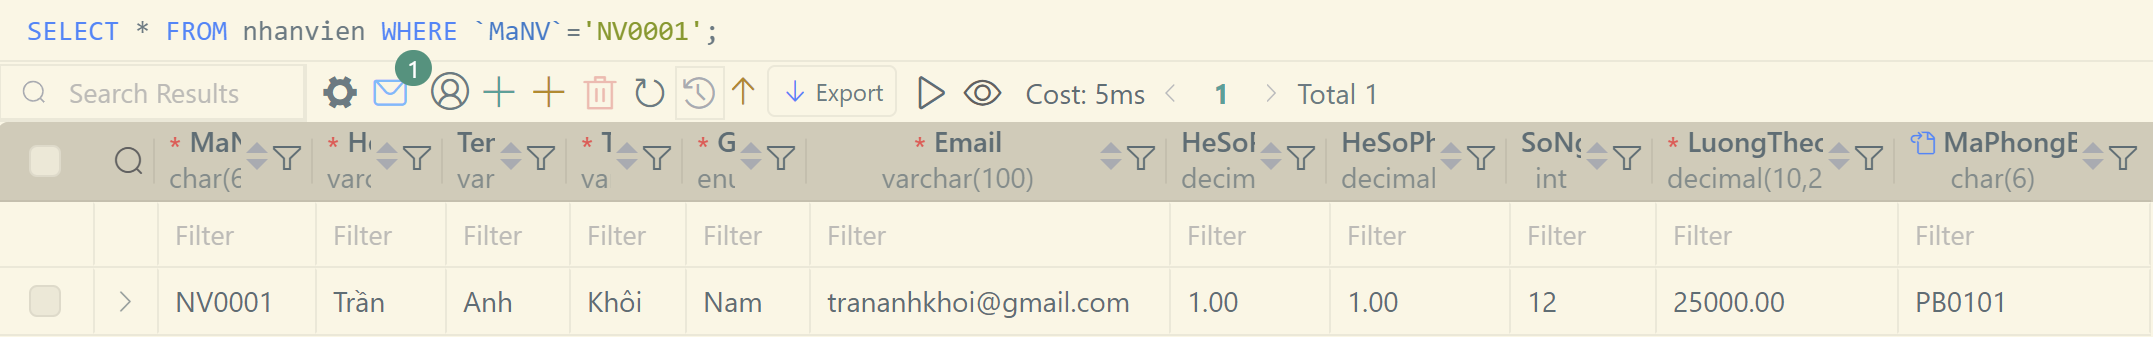
\includegraphics[width=\linewidth]{content/images/SuaNhanVien_After.png}
    \caption{Kết quả sau khi thành công sử dụng thủ tục SuaNhanVien, email đã được thay đổi}
    \label{fig:SuaNhanVien_After}
\end{figure}


\newpage
\subsubsection{Thủ tục DELETE}
\textbf{Mô tả thủ tục:} Thủ tục có nhiệm vụ thực hiện lệnh xóa một thực thể trong hệ thống. Thủ tục hoạt động như sau: qua MaNV được cung cấp, thủ tục tiến hành tìm kiếm và xóa các thực thể có liên quan đến nhân viên đó ở mọi bảng trong hệ cơ sở dữ liệu.

\textbf{Input:} 
\begin{itemize}
    \item [--] Tham số p\_MaNV, có kiểu \texttt{CHAR(6)}
\end{itemize}

\textbf{Output:} Không có.

\begin{minted}{mysql}
    -- Thủ tục xóa nhân viên
    DROP PROCEDURE IF EXISTS XoaNhanVien //
    CREATE PROCEDURE XoaNhanVien(
        IN p_MaNV CHAR(6)
    )
    BEGIN
        -- Xóa dữ liệu liên quan từ các bảng con trước
        DELETE FROM LanRaVao WHERE MaNV = p_MaNV;
        DELETE FROM BangChamCong WHERE MaNV = p_MaNV;
        DELETE FROM LichLamViec WHERE MaNV = p_MaNV;
        DELETE FROM NhanVienThamGiaDuAn WHERE MaNhanVien = p_MaNV;
        DELETE FROM NguoiPhuThuoc WHERE MaNV = p_MaNV;
        DELETE FROM Sdt_NhanVien WHERE MaNV = p_MaNV;
        DELETE FROM BangLuong WHERE MaNV = p_MaNV;
    
        -- Xóa nhân viên từ bảng cụ thể
        DELETE FROM NhanVienBanThoiGian WHERE MaNV = p_MaNV;
        DELETE FROM NhanVienToanThoiGian WHERE MaNV = p_MaNV;
    
        -- Cuối cùng, xóa nhân viên từ bảng chính
        DELETE FROM NhanVien WHERE MaNV = p_MaNV;
    END //
\end{minted}

\newpage
Câu lệnh thực thi thủ tục thành công
\begin{figure}[H]
    \centering
    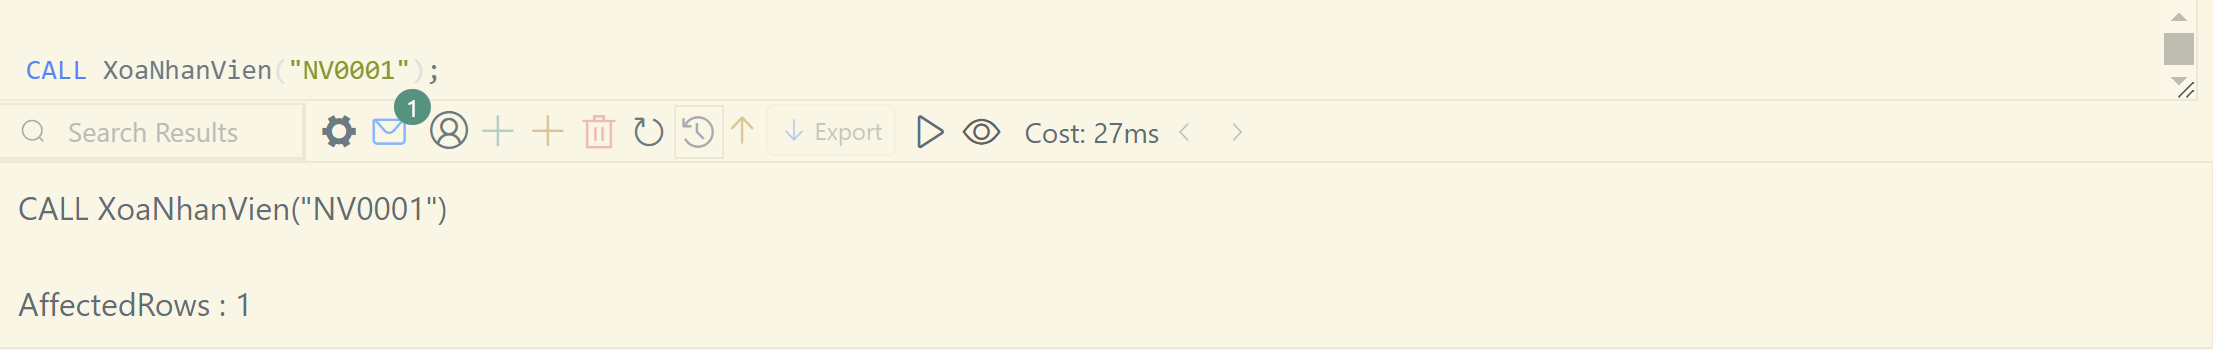
\includegraphics[width=\linewidth]{content/images/XoaNhanVien_ThanhCong.png}
    \caption{Thực thi thủ tục XoaNhanVien thành công}
    \label{fig:XoaNhanVien_ThanhCong}
\end{figure}

Kết quả thực thi thủ tục XoaNhanVien, khi truy vấn bảng NhanVien với MaNV là "NV0001" thì không cho kết quả.
\begin{figure}[H]
    \centering
    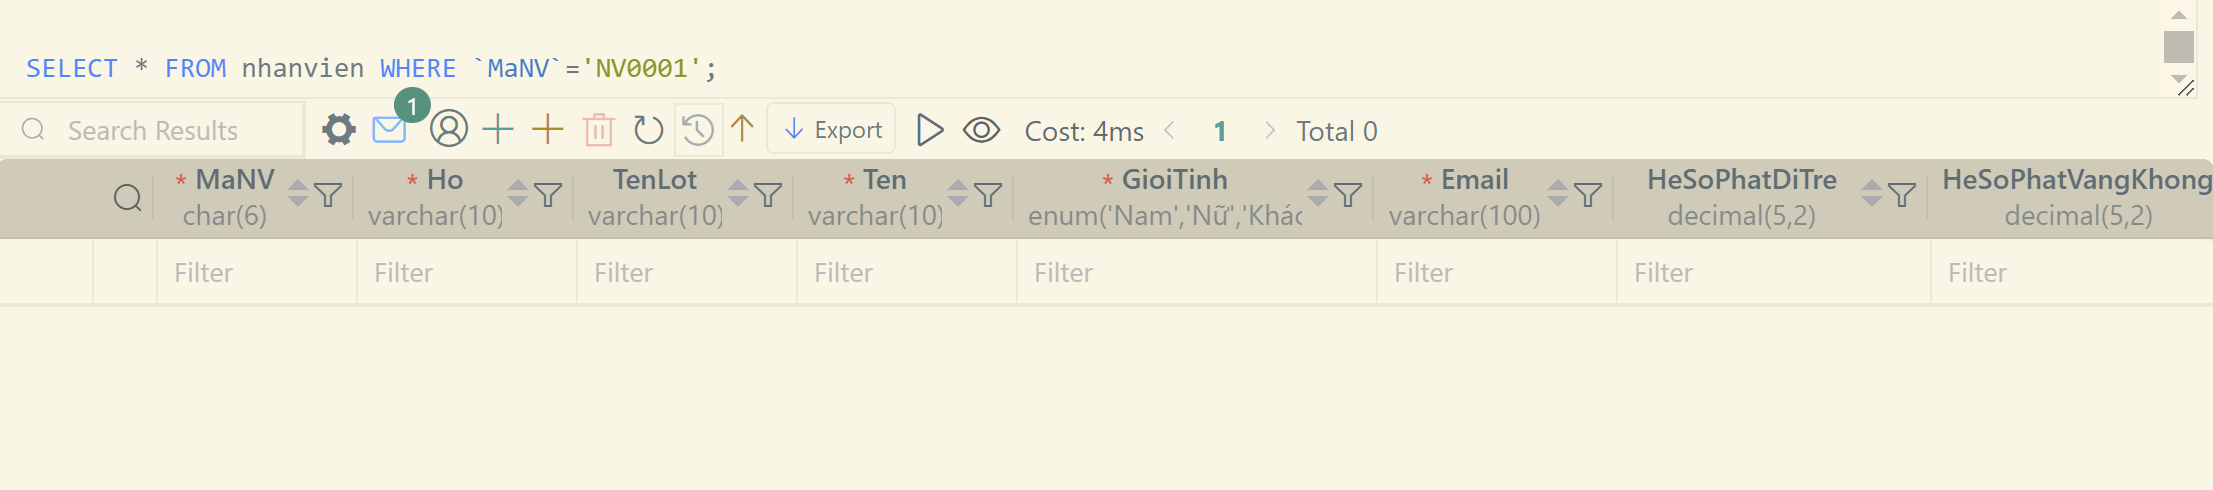
\includegraphics[width=\linewidth]{content/images/XoaNhanVien_After.png}
    \caption{Kết quả thực thi thủ tục XoaNhanVien}
    \label{fig:XoaNhanVien_After}
\end{figure}

\newpage
